\section{ FaceLift:  Specifics}
We try to elaborate on the particular training 
Looking at diminished classifier performance for city only images augmented using translation and rotation, the question arises, which images are worth augmenting, and which images, when augmented, add more noise to the system than information. 
On these lines, we look at a sample set of images, which are augmented at varying distances of 0, 20, 40 and 60 meters. A simple similarity metric of cosine angle between Fc7 features of images (Placesnet) is used to computationally validate similarity. 
Figure \ref{fig:normedCosine} suggests that on an average across the sample set, the similarity tends to go down (Angle tends to increase) as you go farther from the original image. But all is not lost as the standard deviation suggests that even at 60 meters, you may find images which are similar at par to the one taken at 0 meters translations.


\begin{figure}[ht]
	\centering
	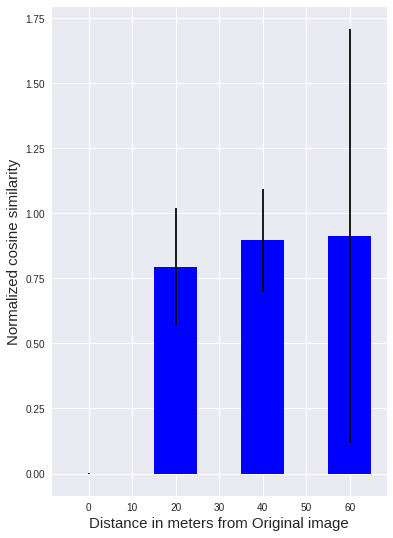
\includegraphics[width=0.5\columnwidth]{Plot/Normed_cosineSim_Aug_5000.png}
	\caption{Variation of similarity angle (radians) with deviations}
	\label{fig:normedCosine}
\end{figure}



The question arises that can we detect this augmentability criteria in an image before hand. To do this, we use the same sample and classify the whole sample set into two classes
We divide the images into two sets. 
\begin{itemize}
	\item $set A$: Images where the median similarity angles between augmented images and the original image are less than median cosine similarity angles for 0 meter set across all images. 
	\item $set B$: Images where the angles are more than 0 meters set. 
\end{itemize}

 $setA$ is as expected a minority set compared to $setB$, hence we manually balance them by selecting less samples from $setB$. To analyse types of scenes that fall in each set, we first get the top 5 labels for each image for both sets, and find the prevalence of labels in both the sets. this is done simply by subtracting $\{l_i   \forall i \in A\}$ where $l_i$ is the label. The resulting set of label,Count pairs are essentially how common or uncommon is a particular label in $setA$ compared to $setB$

\begin{figure}[ht]
	\centering
	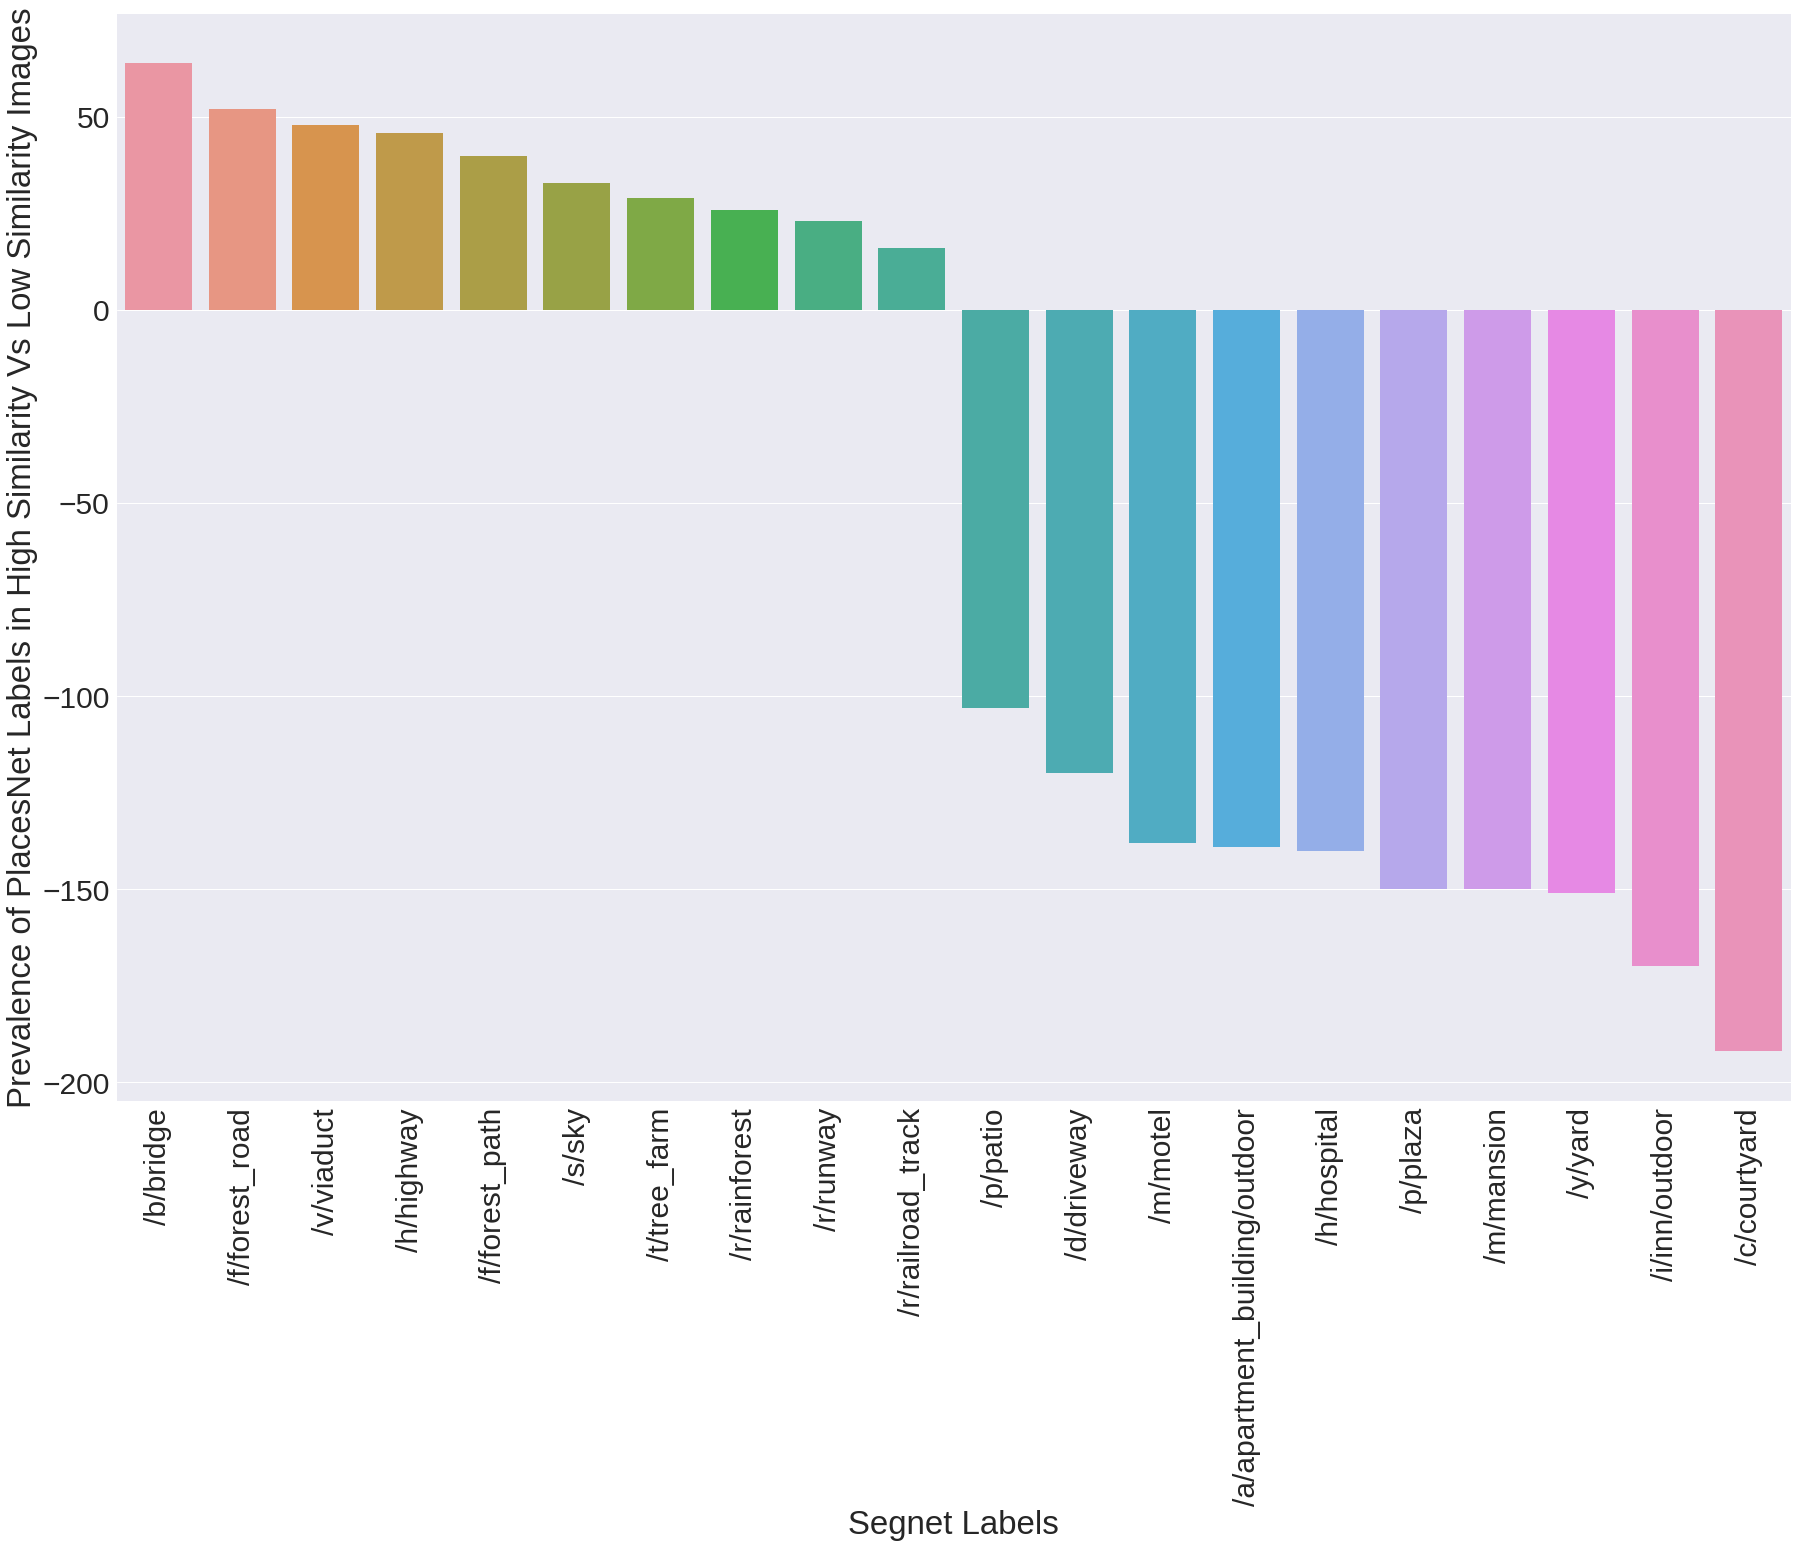
\includegraphics[width=\columnwidth]{Plot/SimilarityPlacesPrevalence.png}
	\caption{Prevalence plot of types of scenes prevalent in Similar images compared to dissimilar ones.}
	\label{fig:augmentationSimilarity}
\end{figure}

The resulting prevalence of scene types can be seen in Fig \ref{fig:augmentationSimilarity}. The plot shows that there are certain scenes which are more open like highways, fields and bridges which don't change despite translation. On the other had there are more urban scenes like gardens, residential neighbourhoods , plazas and skyscrapers which are intuitively more sensitive to change in perspective by translation. 
To test the validity of this observation, we do a small test, which augments a very small set of images taken from the three major cities on the eastern US coast. We select Washington-DC , New York and Boston for our experiment. We end up with just 5300 images from these three cities (and which have high trueskill confidence). This number is too small to train a binary beauty classifier and naturally the training ends up in an overfit model. So we do two seperate training cycles for these images, one where we take all the augmented images for each and every single image from the set of 5300 images. The other training is done on augmentation which is decided based on the most prevalent scene types found from the previous analysis from Fig. \ref{fig:augmentationSimilarity}. For reference, the best performing model which we have trained on all the high confidence images, augmented with just change in camera heading yields an accuracy of 74\%. The model trained on the first experiment plateaus at a modest accuracy of 64\%. The model trained on the second experiment with smart augmentation yields an accuracy of 68\%. This hints at the usefulness of this augmentation trick


\begin{table}[h]
	\centering
	\begin{tabular}{|c|c|}
		\hline
		\textbf{Policy} & \textbf{Accuracy (Percentage)}\\
		\hline
		No augmentation (3k images)  & Overfit \\
		\hline
		Rotation across 5 angles (15k images) & 64 \\
		\hline
		Rotation + translation at 4 distances  & 63 \\
		\hline
		Rotation + Smart Translation & 68 \\
		\hline
		
		\hline
	\end{tabular}
	\caption{Performance differences based on different augmentation policies, for the 3 Cities data}
	\label{tab:augmentation}
	%        \vspace{-5mm}
\end{table}


\subsection{Pipeline Validation}
The overall design of the pipeline is such that it transforms an image according to the trained model, either into a beautiful or an ugly version of itself. In the following sections, we will try to understand the changes 
that the model promotes for the sense of beauty or ugliness. However, before we delve into that, we need to understand how relevant are these transformations. Because beauty is a subjective opinion, 
we take help of crowdsourcing to understand how much do real humans agree with the pipeline's transformations.
We randomly select 200 images, 100 from the fringe beauty area of the distribution and 100 from the ugly area. These images are then transformed into the opposite side of the spectrum. So a beautiful image would be transformed into an ugly image and vice versa. Then we design an Amazon Mechanical Turk experiment, where we ask the turkers to choose the beautiful image between the original and the transformed images. We make sure that we have at least 3 votes on each image comparison, there by allowing us to choose majority voting. The results show that over all , the Turkers agree with the model \textbf{76.5\%} of the time. Besides the over all agreement, the turkers agree \textbf{70\%} of the time with beautification transforms and \textbf{86\%} of the time with ugly-fication transforms.
These crowd sourcing findings suggest that our model is doing a better job at transforming images into an uglier version of themselves , that transforming them into a beautiful version. Nevertheless the over all results are much better for the first iteration with noisy and limited data. This motivates and stabilizes our further analysis of explainablily of the underlying model using urban design metrics.